%\documentclass[aps,amssymb,preprint,a4paper,dvips]{revtex4}
\documentclass[12pt,twocolumn]{iopart}

%\usepackage[latin1]{inputenc}
\usepackage[T1]{fontenc}
\usepackage[english]{babel}
\usepackage{braket}
\usepackage{epsfig}
\usepackage{graphicx}
\usepackage{xcolor}
\usepackage{placeins}
%\usepackage{amsmath,amsfonts,amssymb}
\usepackage{iopams}
\usepackage{dsfont}
\usepackage{booktabs}
\usepackage{multirow}
\usepackage{units}
%\usepackage{natbib}

%Finde die Bilder
%\graphicspath{{./pics/}} 

% Alphabetic counting in footnotes
\renewcommand{\thefootnote}{\alph{footnote}} 

% Captions over full width

%\usepackage{caption}
%\captionsetup[figure]{format=plain, justification=raggedright, singlelinecheck=false, font=footnotesize, labelfont=bf}
%\captionsetup[table]{position=top, format=plain, justification=raggedright, singlelinecheck=false, font=footnotesize, labelfont=bf}

\begin{document}




\setlength{\tabcolsep}{12pt}

% Define some colour
\definecolor{diplom1}{rgb}{0.0 0.4 1.0}
\definecolor{diplom2}{rgb}{0.0 0.0 0.6}
\definecolor{diplom3}{RGB}{153,0,0} %unirot

%\title[Non-nearest Neighbour ICD in Clusters]{Non-nearest Neighbour ICD in Clusters: A Way to Distinguish Icosahedral
%       and Cuboctahedral Clusters?}
\title[Non-nearest Neighbour ICD in Clusters]{Non-nearest Neighbour ICD in
       Clusters}

\author{E Fasshauer}
\address{Centre for Theoretical and Computational Chemistry,
         Department of Chemistry, University of Troms\o,
         -- The Arctic University of Norway, N-9037 Troms\o, Norway}

\eads{\mailto{elke.fasshauer@uit.no}}


\date{\today}

\begin{abstract}
 \begin{abstract}
Interatomic Coulombic Decay (ICD) is an electronic decay process of
excited, ionized systems. It has been shown to occur in a multitude of small
and large systems.
The effects of more than one possible decay
partner are discussed in detail illustrated by simulated ICD electron spectra
of NeAr clusters and pure Ne clusters.
Hereby, the mostly underestimated contribution of decay with
non-nearest neighbours is highlighted. In the neon clusters, the lifetime of the
bulk atoms is found to be in excellent agreement with experiment, while the
lifetimes of the surface atoms differ significantly. Hence, the experimental
lifetime can not purely be explained by the effect of the number of
neighbours.

We propose the possibility to investigate the transition from
small clusters to the solid state by using the ICD electron spectra to
distinguish between icosahedral and cuboctahedral cluster structures.
\end{abstract}

\end{abstract}

\pacs{33.50.Hv, 33.70.Fd, 33.70.Jg, 34.80.Dp, 36.40.-c, 36.40.Mr}
\submitto{New Journal of Physics}

\maketitle


\section{Introduction}

The Interatomic Coulombic Decay (ICD) is an electronic decay process of an atom or
molecule (a unit) involving atoms or molecules of the environment. After an
ionization from the sub-valence region of a unit $A$, the vacancy is filled
by an electron of the same unit and the excess energy is transferred to a decay
partner $B$, which subsequently get ionized:

\begin{equation*}
 A^+ + B \rightarrow A^+ + B^+ + e^-_{ICD}  .
\end{equation*}

The two units $A$ and $B$ are both positively charged, repell each other and
thereby undergo a Coulomb explosion. This process was predicted theoretically
\cite{Cederbaum97} and later proven experimentally \cite{Marburger03}. Since then
it has been studied in a multitude of different systems such as small and large
rare gas clusters \cite{many,Fasshauer14_1},
clusters of small molecules \cite{},
quantum dots \cite{Bande13}
and proteins \cite{Harbach13}. Additionally it has given raise to
the investigation of a whole zoo of ICD-like processes (see Ref. \cite{}
and references therein).

In order to undergo an ICD and it to be observable, two criteria have to
be fulfilled: the energy and the coupling criterion. The energy criterion
requires the energy conservation to hold. In case the doubly ionized final
state is higher in energy than the singly ionized initial state, the ICD
is energetically forbidden. The coupling criterion requires the decay
process to be sufficiently efficient to outperform other decay pathways
such as radiative decay by emission of a photon or coupling to the nuclear
degrees of freedom in molecules. The property calculted for this is the
decay width $\Gamma = \frac{\hbar}{\tau}$, which is inversely proportional
to the lifetime $\tau$ and proportional to the decay rate $\frac{1}{\tau}$.

The ICD process was so far mostly discussed for the case of decay partners in
the direct vicinity, because the decay widths with decay partners further away
was considered to be negligible. Therefore, the decay was studied in clusters
up to 13 neon atoms considering the initial ionization of only the central
atom and not the other ones \cite{Santra01_3}. In this study, a higher than
linear dependence of the decay width on the number of neighbours was
observed. A linear dependence would be expected for equally decay partners
at equal distances from the initially ionized atom in the same environment.
Since the decay width in the asymptotic limit shows an 
$1/\omega^{4}_{vp}$-behaviour on the energy of the virtual photon, which
is decreased for a stabilized final state, this additional feature
can be related to
the better energetic stabilization of the doubly ionized
final state in larger clusters \cite{Fasshauer13}.

We showed that decay pathways with decay partners at larger distances need to
be included for larger systems with many decay partners for two reasons:
\begin{enumerate}
 \item In cluster structures more than one pair of units can consist of
       the same atom types and have the same interatomic distance. Hence,
       they are indistinguishable in the spectrum. Since the decay rate
       is proportional to the number of such pairs as well as the peak
       intensity, the peaks stemming from several pairs are favoured
       compared to other ones at similar distances. Therefore, peaks
       stemming from decays with distant decay partners can be visible
       in ICD spectra of clusters. \cite{Fasshauer14_1}
 \item The opening of ICD-like decay channels depend on the interatomic
       distance. A channel being closed at the distance to the most direct
       beighbours might be open for interaction partners at slightly
       larger distances. If this particular decay channel is more efficient
       than other decay channels being open for the decay with direct
       neighbours, it can still be visible in the spectrum or even
       outperform the slower decay pathways and hence they have to be
       taken into account. We have shown this for the case of ICD vs.
       the Electron Transfer Mediated Decay (ETMD3) process in mixed ArXe
       clusters \cite{Fasshauer13,Fasshauer15_2}.
\end{enumerate}
However, this feature of non-nearest neighbour ICD
has so far not been addressed by itself.

Rare gas clusters are favourable test systems for basic features both
from a theoretical and an experimental point of view. Their spherical
symmetry and their very localized orbitals allow for an comparably easy
theoretical description of the decay processes and the gaseous state
of their components allows for a convenient cleaning of the experimental
setup allowing for higher count rates and therefore a higher resolution
of the spectra. However, the structure of the clusters reveals an
interesting matter of research. Small, ideal clusters exhibit an icosahedral
structure while large clusters have a face-centered-cubic (fcc) structure.
It is still unclear at which cluster size the transition from a favourable
icosahedral to an fcc structure is. Numbers in the range of 800--3000 atoms
have been reported. \cite{}
We propose to use the ICD to be a possible tool to differentiate between
icosahedral and fcc cluster structures using the different distance
patterns in the cluster structures.

We will
therefore first discuss the distance dependency of the ICD in general
in section \ref{sec:theory} and then
zoom in on the NeNe ICD part of the ICD spectra of NeAr clusters
\cite{Fasshauer14_1} in section \ref{sec:near}. Here we will discuss the
peaks and their origin in detail and thereby
raise the question, what a \emph{nearest neighbour} is supposed to be. From
our conclusions we propose the possibility to distinguish cluster structures
of ideal icosahedral and fcc structures using ICD spectra in
section \ref{sec:icofcc}.

%\begin{figure}[h]
% \centering
% \includegraphics[width=\columnwidth]{pics/2dim_coincs.eps}\\
% 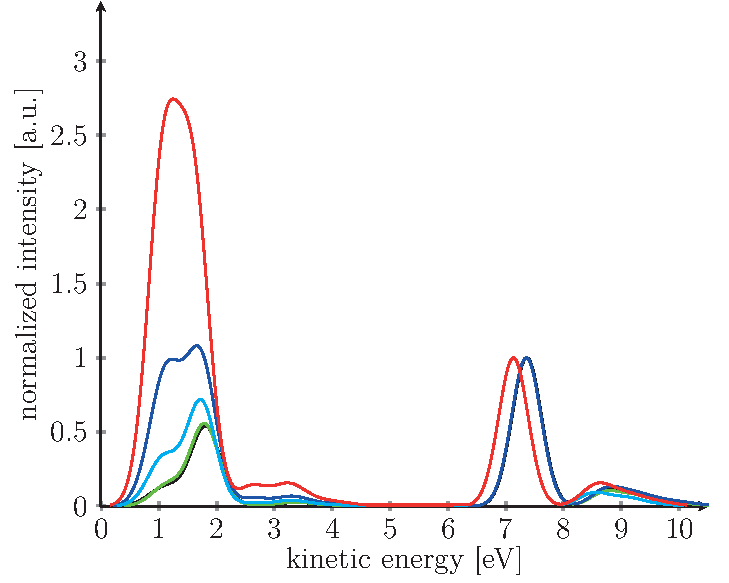
\includegraphics[width=\columnwidth]{pics/NeArcluster_theospecs.pdf}
% \caption{Experimental and theoretical NeAr ICD spectra \cite{Fasshauer14_1}.
%          The experimental spectra were obtained for different cluster expansion
%          conditions and the theoretical spectra were obtained for different
%          underlying cluster structures. In both the NeNe and the NeAr ICD part
%          of the spectrum a main peak and next to it at least one more peak at
%          higher energies are observed. These smaller peaks stem from decays
%          with decay partners at larger distances \cite{Fasshauer13,Fasshauer14_1}.}
% \label{figure:near_spectra}
%\end{figure}

\section{Theoretical Background}
\label{sec:theory}

In roder to simulate the ICD electron spectra for a given cluster structure,
the kinetic energies of the ICD electrons $E_{ICD}$ and the corresponding decay
decay widths of all pairs have to be determined. The ICD electron energies
are given by the differences between the initial state and the final state
energies $E_{in}$ and $E_{fin}$, respectively. The initial state energy
is given by the single ionization potential (SIP) of the sub-valence electron
of the entire system
and the final state energy is given by the double ionization potential (DIP).
In the asymptotic limit, which is a reasonably good approximation for
weakly bound systems, he initial state energy is approximated by the SIP
of the initially ionized unit $X_{in}$ and the final state energy can be
approximated
by the sum over the SIPs of the electron donating unit $X_D$ and the electron
emitting unit $X_E$ ionized in the final state as well as the
Coulomb repulsion between two point charges at the interatomic distance $R$

\begin{align}
 E_{ICD}^\beta &= E_{in}^\beta - E_{fin}^\beta \label{equation:E_sec}\\
 E_{in}        &= SIP(X_{in}) \label{equation:E_in}\\          
 E_{fin}^\beta &= SIP(X_{D}^\beta) + SIP(X_{E}^\beta) + \frac 1R
           \label{equation:E_fin}                . 
\end{align}
Here, $\beta$ denotes the selected decay channel.

Following Wentzel \cite{Wentzel27}, Feshbach\cite{Feshbach58,Feshbach62}
and Fano \cite{Fano61} the decay width is given by

\begin{equation}
 \Gamma_{\beta}(E_{res}) = 2\pi \left|
                           \braket{\Phi_{in}| H_f |\chi_{\beta}}
                           \right|^2   .
\end{equation}
Here, the bound and ionized initial state is described by $\ket{\Phi_{in}}$ and
the final continuum state of a particular decay channel $\beta$ is
given by $\ket{\chi_{\beta}}$.
This challenging description involving both bound and continuum states can
amongst others be achieved by the FanoADC-Stieltjes approach, where a
subset of the $2h1p$ functions within the Algebraic Diagrammatic Construction
(ADC) are used to mimic the final state function $\ket{\chi_{\beta}}$.
By these means calculated discrete energies and corresponding transitions
moments are then used to construct a continuous function, which is evaluated
at the resonance energy approximated by the single ionization potential
corresponding to the initial state $E_{in}$. For a more detailed
description of the method and comparison to other approaches see References
\cite{Averbukh05,Fasshauer15_1} and references therein.

\section{Computational Details}
\label{sec:computational}
The cluster structures used were constructed to have an ideal icosahedral or
face-centered-cubic geometry with optional additional incomplete outermost
shells. These are based on the van der Waals radii for neon
$r_{Ne}=\unit[1.54]{\AA}$
and argon $r_{Ar}=\unit[1.88]{\AA}$ \cite{Bondi64}.
In case of the NeAr clusters two of those
cluster structures from Ref. \cite{Fasshauer14_1} that matched best
with the combination of the argon content in the cluster,
the NeAr-ICD to total
ICD ratio and the peak position of the NeAr-ICD peak were used.
These are $C_{Ar}=3$, $C_{Ne}=1$, $S_{Ne}=7$
for set 3
and $C_{Ar}=2$, $C_{Ne}=1$, $S_{Ne}=13$ for set 5, where $C_{Ar}$ denotes
the edge length of the argon core, $C_{Ne}$ denotes the number of complete
neon shells around the argon core and $S_{Ne}$ denotes the number of 
triangular surfaces additionally covered by neon atoms.


\begin{table}[h]
 \caption{Experimental values for the single ionization potentials
          \cite{Fasshauer14_1}
          used for the estimation of the decay widths.}
 \label{table:exp_input}
 \centering
 \begin{tabular}{lc}
  \toprule
  indicator            &  value \\
  \midrule
  SIP(Ne2s)            &  \unit[47.75]{eV} \\
  SIP(Ne2p)            &  \unit[21.10]{eV} \\
  SIP(Ar3p)$_{c<3}$    &  \unit[15.40]{eV} \\
  SIP(Ar3p)$_{c\ge 3}$ &  \unit[15.20]{eV} \\
  \bottomrule
 \end{tabular}
\end{table}


The calculations to obtain the ICD electron spectra of those cluster
structures were performed with
the program HARDRoC \cite{HARDRoC} using experimental ionization energies shown
in Table \ref{table:exp_input} and curves fitted to the decay width of the
NeNe ICD of Ref. \cite{Averbukh06_1}. With these choices the lifetimes of a
pair at the dimers equilibrium distance are $\tau_{NeNe}= \unit[60]{fs}$ and
$\tau_{NeAr}= \unit[44]{fs}$.

\section{Decay with Decay Partners at Different Distances}

\section{ICD in Clusters}
\label{sec:clusters}

\subsection{NeAr Clusters}
\label{sec:near}
After ionization from the Ne2s, a heteronuclear NeAr cluster can decay
via two competing pathways:

\begin{center}
\begin{tabular}{lcr}
 Ne(2s$^{-1}$) + Ne &$\rightarrow$ & Ne(2p$^{-1}$) + Ne(2p$^{-1}$) + $e^-_{ICD}$\\
 Ne(2s$^{-1}$) + Ar &$\rightarrow$ & Ne(2p$^{-1}$) + Ar(3p$^{-1}$) + $e^-_{ICD}$
\end{tabular}
\end{center}

in which the excess energy gained by filling the Ne2s vacancy is transferred to
either another neon atom or to an argon atom. Since the lifetimes of the
NeNe-ICD and the NeAr-ICD are of the same order of magnitude, both are
visible in the secondary electron spectrum (see Figure 2 of
Ref. \cite{Fasshauer14_1}). The two signals are well separated in energy
and both consist of a main peak and a shoulder at higher kinetic energies
of the ICD electron.
We earlier showed a clear
geometry dependence of peak intensity relation of the NeNe-ICD and NeAr-ICD
and utilized this property to determine the structure of
heteroatomic rare gas clusters \cite{Fasshauer14_1}.

The peak structure of one main peak and a shoulder at higher energies has been
discussed for the NeAr before. Theoretical investigations indicate that the
shape might be caused by different vibrational levels of the NeAr dimer
($v=0,1,2$) being populated prior to the initial ionization, because
the calculated lifetimes of the intermediate states were too short to allow
for nuclear dynamics \cite{Scheit06}.
There, the ratio of the population of the three vibrational levels 10:5:4
was chosen to yield a spectrum close to the experimental spectrum of NeAr
clusters.
However,
recent experimental results of the ICD in the NeAr dimer show a symmetric peak
without a shoulder \cite{OKeeffe14}. In order to explain this, the authors assume
a bond contraction of the Ne$^+$Ar to happen prior to the decay.
This nuclear rearrangement would contradict the
theoretically predicted lifetime of the system and they therefore propose
the prior value to be wrong and give an estimate for a higher lifetime.
We would like to emphasize the possibility that mainly the vibrational
ground state was populated at the temperatures at which the
experiment was conducted and that the theoretically predicted lifetimes are
correct.
Since the shoulder appears in the spectrum of clusters only and not in the
dimer spectra, we interpret these experimental results of the dimer to confirm our
findings, that the shoulder stems from ICD with interaction partners of the
next shell \cite{Fasshauer14_1}.
%This hypothesis is furtherly supported by the fact that
%in the clusters the decay rate scales approximately linearly
%with the number of nearest ineighbour decay partners.
%In other words, the lifetime of the
%singly ionized initial state is only a fraction of the dimer's lifetime and
%therefore, the nuclear motion will be even less important than in the dimer.

In the neon dimer several vibrational states of the ionized initial state are
involved in the decay. \cite{Santra00_1} It has furthermore been shown, that
the experimentally determined lifetime of $\tau_{NeNe}=\unit[150\pm 50]{fs}$
\cite{Schnorr13} is only in agreement with those theoretical lifetime
calculations that explicitly include nuclear dynamics of the intermediate state.
\cite{Schnorr15} However, the early lifetime measurements in neon clusters with
a mean cluster size of $<N>=\unit[900]{atoms}$ show a lifetime of
\unit[30]{fs} for surface atoms and \unit[6]{fs} for bulk atoms. This lifetime
decrease is caused by the possibility to decay with several decay partners.
Nuclear dynamics occur in the range of tens of femtoseconds in the dimer.
Additionally, the driving force for a bond contraction after the initial
ionization is higher in dimers than in clusters, where one bond contraction
usually leads to several bond elongations. Therefore, we consider the influence
of nuclear dynamics on the lifetime to be sufficiently small to be able to
neglect them in clusters in a first description.
\cite{Santra01_3,Ohrwall04}
However, in clusters the nuclear
motion might not be fast enough to play a role due to the manifold of
decay partners and the resulting shortening of the lifetime.
In the following, we will focus on the NeNe-ICD part of the
ICD electron spectra of the NeAr clusters and analyze them in more detail.

\begin{figure}[h]
 \centering
 \includegraphics[width=0.7\columnwidth]{pics/rot.pdf}\\
 \includegraphics[width=0.7\columnwidth]{pics/blue.pdf}
 \caption{ICD spectra for the NeNe-ICD part of the structures of set 3 and
          set 5 of the NeAr clusters in Ref. \cite{Fasshauer14_1}
          plotted as stick spectra.
          The different peak groups resemble different pair types
          within the NeAr clusters. The lowest energy peaks (\textbf{(a)})
          refer to nearest neighbours
          of different shells, the peak group \textbf{(b)} refers
          to nearest neighbours within one shell and the peak group \textbf{(c)}
          refers to next-nearest neighbours between adjacent shells.
          The other peaks contain both peaks stemming from
          pairs within the same shell as well as pairs consisting of atoms
          of different shells.}
 \label{figure:rot_blue}
\end{figure}

In Figure \ref{figure:rot_blue} the ICD electron spectra for the NeNe-ICD
part of heterogeneous clusters are shown as stick spectra
for set 3 and set 5. Hereby, we stick to the naming and the color code of
Ref. \cite{Fasshauer14_1}. Both spectra exhibit a similar pattern of peak groups.
The groups are found around \unit[1.0]{eV} (group \textbf{(a)}),
around \unit[1.7]{eV} (group \textbf{(b)}), around \unit[2.6]{eV}
(group \textbf{(c)})
and from \unit[3]{eV} to \unit[4]{eV}.
The peak groups can be assigned to atom pairs
within the cluster. For group \textbf{(a)} the peaks stem from decays
between two nearest neighbour atoms of two different shells,
while group \textbf{(b)}
stems from the decay partners being nearest neighbours in the same shell.
Group \textbf{(c)} can be assigned to non-nearest neighbours in adjacent shells
and the other peaks stem from a mixture of pairs which cannot unambigiously
be categorized because different kinds of peaks intersect each other.

Obviously, the peak groups have a fine structure which originates from
different positions of the decay partners within a shell (face, egde or vertex).
For the investigated ideal icosahedral structures,
these pairs of group \textbf{(a)}
are from low to high kinetic energies: vertex-vertex, edge-edge, edge-face and
face-face. Due to vibrational broadening of the peaks the experimental observation
of this fine structure is unlikely in neon clusters.

Concluding these findings, there is not neccessarily only one kind of nearest
neighbours in clusters. Even the next-nearest neighbours are closer to
twice the interatomic distance of the closest pair with an open decay channel.
Therefore, also non-nearest decay partners need to be taken into account
in order to simulate ICD spectra of clusters.
It can be considered safe to neglect decay partners at sufficiently larger
distances than twice the closest interatomic distance between decay partners
with open channels.


\subsection{Neon clusters: Icosahedral vs. Cuboctahedral Structure of Clusters}
\label{sec:icofcc}
We study two cluster structures of \unit[55]{atoms} each, where one has an
idealized icosahedral and the other one has an idealized cuboctahedral structure.
They hence consist of 13 core and 42 surface atoms each. It was predicted
theoretically and proven experimentally that the lifetimes of ionized bulk atoms
is shorter than of ionized surface atoms due to the smaller number of direct
neighbours of surface atoms. \cite{Santra01_3,Ohrwall04}
The experimentally determined lifetimes are
$\tau_{surf} = \unit[30]{fs}$ and $\tau_{bulk} = \unit[6\pm 1]{fs}$.
For our \unit[55]{atom} cluster the decay widths and lifetimes are listed in
Table \ref{table:lifetimes}.

\begin{table}[h]
 \centering
 \caption{Calculated decay widths and lifetimes of bulk and surface atoms
          for icosahedral and cuboctahedral clusters of 55 atoms.}
 \begin{tabular}{llrr}
  \toprule
               &                            & $\Gamma$ [meV] & $\tau$ [fs]\\
  \midrule
   \multirow{2}{*}{icosahedral}   & bulk    & 125            & 5.3 \\
                                  & surface &  67            & 9.8 \\
  \midrule
   \multirow{2}{*}{cuboctahedral} & bulk    & 140            & 4.7 \\
                                  & surface &  78            & 8.4 \\
  \bottomrule
 \end{tabular}
 \label{table:lifetimes}
\end{table}

For both the icosahedral and the cuboctahedral cluster structures the lifetimes
of the bulk atoms are in excellent agreement with experiment.
However, the theoretical lifetimes of the surface atoms are significantly
smaller than the experimental lifetime. Assuming that the
experimental lifetimes are correct, we have to consider three error sources:
1. the nuclear motion excluded in our approach, 2. the different cluster sizes,
and 3. a different stabilization of charges between the
inner-valence ionized and the outer-valence ionized atom compared to the bulk.
In small clusters, the number of face surface atoms is small compared to the
number of edge and vertex atoms in the surface. The larger the clusters are,
the larger is the relative number of the surface atoms. These surface atoms
in face positions have more direct neighbours than atoms in vertex positions.
Therefore, our estimated lifetime of the average surface atoms in the small
clusters should be slightly larger than in larger clusters. A pure structure
effect does not explain the difference between the experimental and the
theoretical results.

It remains to discuss the influence of the different charge stabilizations of
inner- and outer-valence vacancies. The decay width is proportional to
$\frac{1}{\omega_{vp}^4}$ where the energy of the virtual photon ($vp$) is given
by

\begin{equation}
 \omega_{vp} = SIP(X_{in}) - SIP(X_D)   .
\end{equation}

If the stabilization difference of the inner-valence vacancy between the bulk
and the surface atoms is larger than the corresponding difference of
the outer-valence
vacancy, the transferred energy is increased in case of the surface atoms
($\omega_{vp,surf} > \omega_{vp,bulk}$). As a consequence, the decay width
is decreased and the lifetime is increased. Unfortunately, only the initial
state energy differences are to be found in the literature \cite{Ohrwall04}.
Hence, a validation of this cause is currently not possible.


Before discussing the ICD spectra  of the icosahedral and cuboctahedral
cluster structures shown in Figure \ref{figure:reinNe}, we would like to
recall that clusters with an icosahedral structure
have shorter interatomic distances between shells than within the same
shell.
In terms of the ICD, different groups of nearest neighbours exist,
one within the same shell and one
between adjacent shells. This is characteristic for icosahedral cluster
structures. Cuboctahedral cluster structures on the other hand are characterized
by only one interatomic distance. 
Therefore, icosahedral cluster structures should be distinguishable from
cuboctahedral clusters by the number of peaks, which can be seen in Figure
\ref{figure:reinNe}.

\begin{figure}[h]
 \centering
 \includegraphics[width=\columnwidth]{pics/reinNe}
 \caption{ICD spectra of pure neon clusters consisting of 55 atoms in
          icosahedral and cuboctahedral structure. In clusters with an
          ideal cuboctahedral structure
          all interatomic distances are the same and hence only one peak
          for each shell around any atom in the cluster is to be expected.
          In ideal icosahedral clusters the interatomic distances between atoms
          within the same shell and between atoms in neighbouring atoms
          are different. Therefore two peaks for interactions partners
          at different distances can be expected. This feature might
          help to experimentally identify the underlying structure of clusters.}
 \label{figure:reinNe}
\end{figure}

Two experimental ICD electron spectra of clusters
with a mean cluster size $<N>$ between 47 and 512 atoms
are available in the literature.
\cite{Marburger03,Barth06_2} 
The first experimental spectrum shows a very
broad ICD electron peak without an unambiguously assignable peak structure,
whereas the later results show a main peak of ICD electrons and a smaller peak
at slightly higher kinetic energies (at around \unit[3]{eV})
that was not even assigned to be an ICD peak in the original work. This peak
corresponds to the decay with non-nearest neighbours in the adjacent shell.
However, a further peak
structure is not visible.

Whether or not the cluster structures would be distinguishable in experiment
will depend on the vibrational broadening of the peaks, the experimental
resolution and difference of the interatomic distances
and hence the energy difference of the peaks in the spectrum of the
icosahedral structure. In this proof-of-principle discussion
we chose neon clusters for comparison with experiment but for the distinction
of cluster structures it might be recommendable to choose atoms with larger
internuclear distances in clusters.


\section{Summary}
\label{sec:summary}

We have discussed two of the three aspects one needs to take into account
to simulate the ICD spectrum of rare gas clusters in detail. Due to the nature
of clusters, a neon atom ionized in the inner-valence will have several decay
partners at different distances. The larger the interatomic distance the higher
is the kinetic energy of the ICD electrons which will yield a multitude of
peaks in the spectrum. These are then weighted by the decay width, which
depends on the interatomic distance of the decay partners but also needs
to be scaled by the number of pairs of the same distance.
The manifold of all different decay events will then yield the spectrum.

When applying these apsects to cluster structures, one finds that not only
the nearest neighbours contribute to the spectrum, but several other decay
partners do as well. Decay partners until a distance of at least twice the
distance of the clostest decay partners should be taken into account.
In clusters with an icosahedral cluster structure this is especially important
because the smallest interatomic distance between atoms of the same and atoms
of different layers is different, but both distances are comparable.
This leads to a different number of peaks in the spectra which might help to
differentiate between clusters of icosahedral and cuboctahedral cluster structure.



\ack

%\begin{acknowledgements}
Funding from the Research
Council of Norway through a Centre of Excellence Grant (Grant No.\ 179568/V30)
is gratefully acknowledged.
%\end{acknowledgements}


\eject
\section*{References}
\bibliographystyle{unsrt}
\bibliography{theolit}


%%%%%%%%%%%%%%%%%%%%%%%%%%%%%%%%%%



\end{document}
